\lecture{19}{2025-04-29}{Error Correction}{}


\begin{parag}{Point to point communication system}
    
\end{parag}


\begin{parag}{Motivation Chanel Model}
    \begin{itemize}
        \item The internet often drops packets due to congestion
        \item Not all the bits on a storage device can be retrieved
        \item \important{Wireless signals are very noisy}
    \end{itemize}
    We consider two types of channel models:
    \begin{center}
        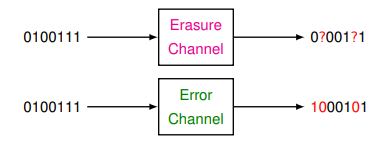
\includegraphics[scale=1]{12025-04-29.png}
    \end{center}
    So for the first $0$ let us say we throw a dice, if the outcome is $6$, we will replace the outcome by a question mark or we won't. Therefore, here we can say that the erosion probability is $\frac{1}{6}$.\\
    However maybe the eraser is not random, maybe someone who know what we're gonna do (the algorithm to find the erasure) will find the one that will be a question mark.
\\
Here the channel input alphabet is not necessarily binary.\\
We can take for the alphabet $\mathcal{A} = \{0, 1, 2, 3, 4\}$ and works with this.
\end{parag}
\begin{parag}{Erasure Weight}
    \begin{definition}
    We define the \important{erasure weigh} $p$ (resp, \important{error weight $p$}) as the total number of erasures (resp. errors).
    \end{definition}
    
    For example if we take the erasure channel from before, $p= 2$.
\end{parag}
\begin{parag}{Channel coding to deal with erasures}
    Here this is the beginning of every algorithm for channel coding which goes:\\
    Suppose that the source outputs $2$ bits, and we store them as is (no channel coding):
\begin{center}
    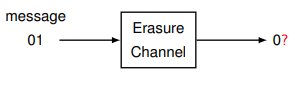
\includegraphics[scale=1.2]{22025-04-29.png}
    
\end{center}
f any bit is erased, there is no way to determine the original message (all hypothese are equally possible).\\
So the goal here is the put redundancy, the goal is the create a redundancy that match exactly the message. The reduncancy serves to deal with the back eyes (i don't rembeber).\\
So first we got rid of redundancy, we encrypt, and the finaly we add back in redundancy (which is not the same as the one we got rid off).
\\    
So first we got rid of redundancy, we encrypt, and the finaly we add back in redundancy (which is not the same as the one we got rid off).
\\
Now suppose that we do channel coding like this:
\begin{center}
    \includegraphics[scale=1]{32025-04-30.png}
\end{center}
The channel output is not a valid codeword. The decoders recognizes it, and assumes that the transmitted codeword is the one that agrees in most position with the observed channel output.
\end{parag}
\begin{parag}{We study only block codes}
    The above is an $\left(n, k\right)$ \important{block code} with $n= 6$ and $k =  2$: each $k$ source symbols are substituted by $n$ channel symbols over the same alphabet.\\
    Since the alphabet is $\{0, 1\}$, we call it a \important{binary} $\left(n, k\right)$ block code.
    
\end{parag}

\begin{parag}{Example}
    The following is a convolutional encoder: every encoder input symbol produces two encoder output symbols.\\
    The output pair produced at any given time is a linear function of the corresponding encoder input and encoder state (the previous two inputs).
    \begin{center}
        \includegraphics[scale=0.9]{42025-04-30.png}
    \end{center}
    

    
\end{parag}
\begin{parag}{Terminology}
    \begin{itemize}
        \item The code $\mathcal{C}$ is the set of codewords 
        \item A codeword $c$ is an element of $\mathcal{A}^n$. (the alphabet $\mathcal{A}$ is $\left\{0, 1\right\}$ in our example)
        \item The block-length is $n$
        \item Each codeword carries $k = \log_2\left|\mathcal{C}\right|$
        \item The rate is $\frac{k}{m}$ bits per symbol
    \end{itemize}
    
    
\end{parag}
\begin{parag}{Hamming distance}
    \begin{definition}
    The \important{Hamming distance $d\left(x, y\right)$} between two $n$-tuples $x$ and $y$ is the number of positions in which they differ.
    \end{definition}
    \begin{subparag}{Example}
        \begin{itemize}
            \item $x = \left(101110\right)$ ,  $y = \left(100110\right)$, $d\left(x, y\right) = 1$
            \item $x = \left(0427222\right)$, $y = \left(1227986\right)$, $d\left(x, y\right) = 5$
        \end{itemize}
        
        
    \end{subparag}
    
\end{parag}
















